\subsection{m5 family}
The first set of experiments will be conducted on an m5 dedicated host. This host features either the 
1st or 2nd generation Intel Xeon Platinum 8000 Series processor, namely Skylake-SP or Cascade Lake 
\cite{aws_m5_instances}. The following table provides an overview of the 
different instance types that belong to this family. 
\begin{table}[H]
\centering
\begin{tabular}{lcc}
\hline
\textbf{Instance Size} & \textbf{vCPU} & \textbf{Memory (GiB)} \\
\hline
m5.large     & 2  & 8    \\
m5.xlarge    & 4  & 16   \\
m5.2xlarge   & 8  & 32   \\
m5.4xlarge   & 16 & 64   \\
m5.8xlarge   & 32 & 128  \\
m5.12xlarge  & 48 & 192  \\
\hline
\end{tabular}
\caption{m5 Instance Specifications \cite{aws_m5_instances}}
\end{table}
\noindent
The m5 dedicated host used the 2nd-generation Intel CPU in all our experiments. 
We repeated the benchmarks using hosts running on the 1st-generation CPU and we received the same
behavior, which excludes variation caused by hardware heterogeneity. 
For our first experiment, we used 2xlarge instances, each featuring 8vCPUs and 32 GiB RAM. 
The maximum number of nodes is 12. The results can 
be seen in Figure \ref{fig::m5.2xlarge_busy}

\begin{figure}[H]
\centering
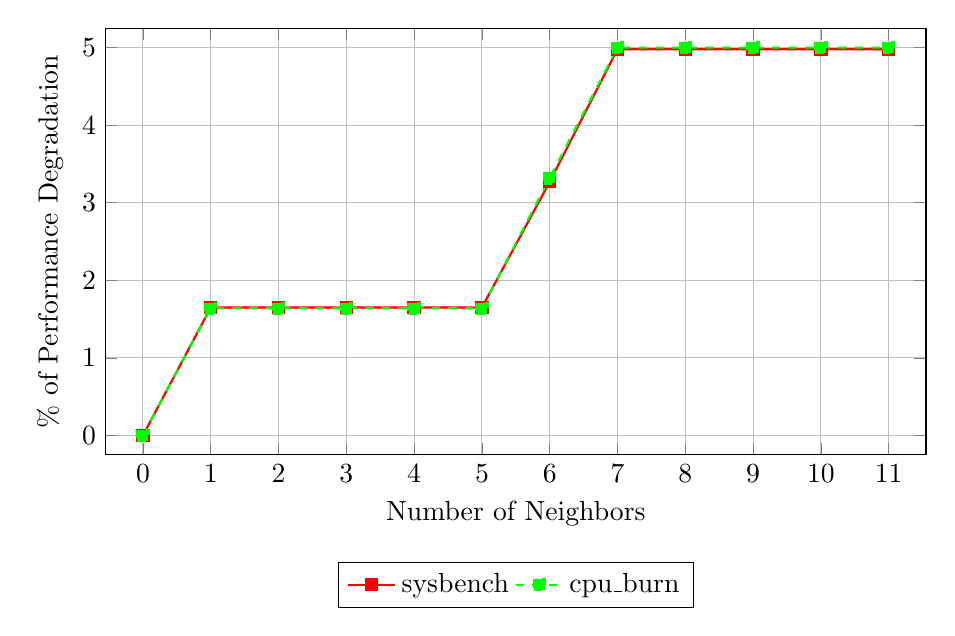
\begin{tikzpicture}
\begin{axis}[
    width=12cm,
    height=7cm,
    xlabel={Number of Neighbors},
    ylabel={\% of Performance Degradation},
    grid=both,
    xtick={0,...,11},
    enlargelimits=0.05,
    legend style={at={(0.5,-0.25)}, anchor=north, legend columns=2}
]


\addplot[
    color=red,
    mark=square*,
    thick
] coordinates {
    (0, 0)
    (1, 1.65)
    (2, 1.65)
    (3, 1.65)
    (4, 1.65)
    (5, 1.65)
    (6, 3.27)
    (7, 4.98)
    (8, 4.98)
    (9, 4.98)
    (10, 4.98)
    (11, 4.98)
};

\addplot[
    color=green,
    mark=square*,
    dashed,
    thick
] coordinates {
    (0, 0)
    (1, 1.64)
    (2, 1.64)
    (3, 1.64)
    (4, 1.64)
    (5, 1.64)
    (6, 3.32)
    (7, 5)
    (8, 5)
    (9, 5)
    (10, 5)
    (11, 5)
};
\addlegendentry{sysbench}

\addlegendentry{cpu\_burn}


\end{axis}
\end{tikzpicture}
\caption{Effect of adding busy neighbors on the CPU speed of the sysbench and cpu\_burn command on the 
test node using m5.2xlarge instances}
\label{fig::m5.2xlarge_busy}
\end{figure}
\noindent
We notice a very similar degradation pattern for the two tools we used.
Adding the first neighbor added a performance degradation of  1.6\% on our test node. The runtime then 
remained constant for the next four neighbors. Afterwards, the sixth neighbor degraded the performance
further to 3.3\%. The seventh neighbor introduced the last witnessed decrease in the performance to 
reach 5\% in both experiments. \\ 
This experiment alone does not allow us to pinpoint the reason behind the performance degradation.
Potential reasons could be physical core co-location between the neighbors and the test node or 
hypervisor overhead. The latter is very unlikely, as the Nitro system, along with hardware-assisted 
virtualization should introduce a very small overhead. 
We repeat the same experiment but adding idle VMs. 
Figure \ref{fig::m5.2xlarge_idle} summarizes the results. 

\begin{figure}[H]
\centering
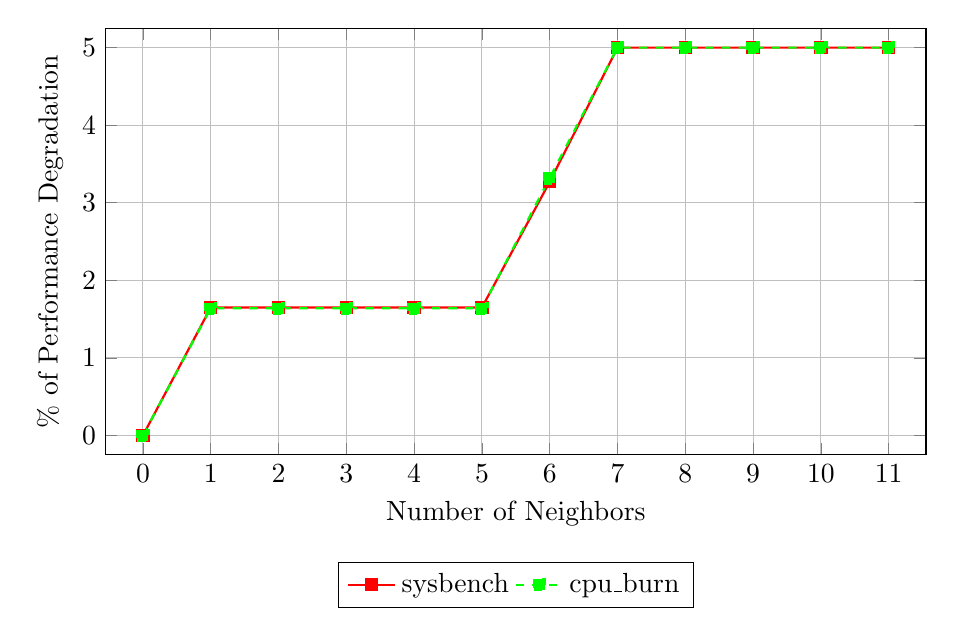
\begin{tikzpicture}
\begin{axis}[
    width=12cm,
    height=7cm,
    xlabel={Number of Neighbors},
    ylabel={\% of Performance Degradation},
    grid=both,
    xtick={0,...,11},
    enlargelimits=0.05,
    legend style={at={(0.5,-0.25)}, anchor=north, legend columns=2}
]


\addplot[
    color=red,
    mark=square*,
    thick
] coordinates {
    (0, 0)
    (1, 1.65)
    (2, 1.65)
    (3, 1.65)
    (4, 1.65)
    (5, 1.65)
    (6, 3.27)
    (7, 5)
    (8, 5)
    (9, 5)
    (10, 5)
    (11, 5)
};

\addplot[
    color=green,
    mark=square*,
    dashed,
    thick
] coordinates {
    (0, 0)
    (1, 1.64)
    (2, 1.64)
    (3, 1.64)
    (4, 1.64)
    (5, 1.64)
    (6, 3.32)
    (7, 5)
    (8, 5)
    (9, 5)
    (10, 5)
    (11, 5)
};
\addlegendentry{sysbench}

\addlegendentry{cpu\_burn}
\end{axis}
\end{tikzpicture}
\caption{Effect of adding idle neighbors on the CPU speed of the sysbench and cpu\_burn command on the test node using m5.2xlarge hosts} 
\label{fig::m5.2xlarge_idle}
\end{figure}
\noindent
We notice the exact same degradation pattern of the earlier experiment. This result is unexpected
and undermines the hypothesis that the performance degradation is due to physical core co-location between the different 
tenants as we would have expected the effect to be less pronounced when adding idle VMs. \\
To explore this further, we repeat the experiment using m5.large instances, of which the dedicated host can 
provision 48. The results of our experiment can be seen in Figure \ref{fig::m5.large}. In this 
case as well, adding busy or idle neighbors provided the exact same results.  

\begin{figure}[H]
\centering
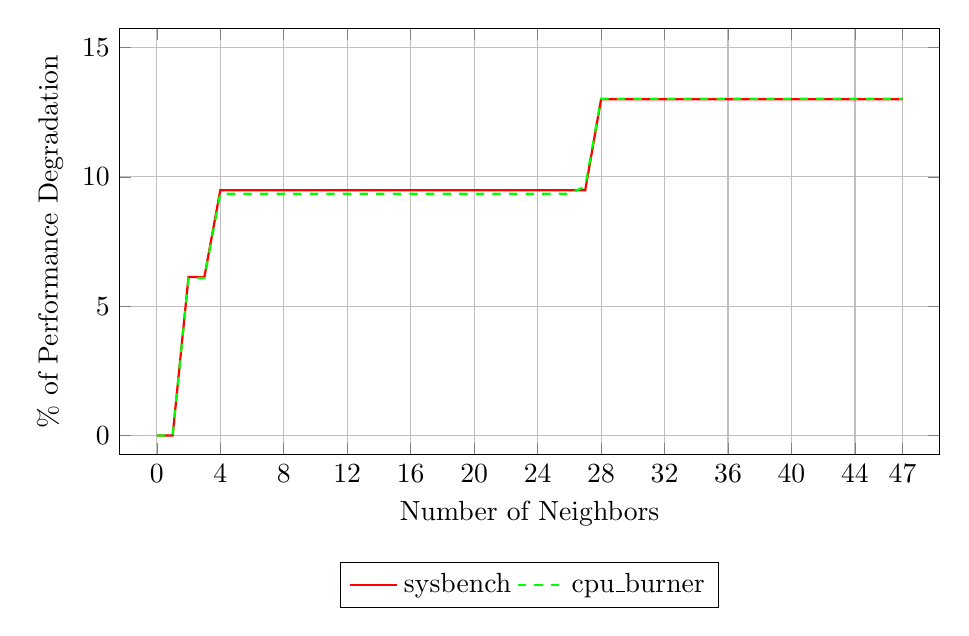
\begin{tikzpicture}
\begin{axis}[
    width=12cm,
    height=7cm,
    xlabel={Number of Neighbors},
    ylabel={\% of Performance Degradation},
    grid=both,
    ymax=15, 
    xtick={0,4,8,12,16,20,24,28,32,36,40,44,47},
    enlargelimits=0.05,
    legend style={at={(0.5,-0.25)}, anchor=north, legend columns=2}
]

\addplot[
    color=red,
    thick
] coordinates {
    (0, 0.00)
    (1, 0.00)
    (2, 6.13)
    (3, 6.13)
    (4, 9.48)
    (5, 9.48)
    (6, 9.48)
    (7, 9.48)
    (8, 9.48)
    (9, 9.48)
    (10, 9.48)
    (11, 9.48)
    (12, 9.48)
    (13, 9.48)
    (14, 9.48)
    (15, 9.48)
    (16, 9.48)
   (17, 9.48)
   (18, 9.48)
   (19, 9.48)
   (20, 9.48)
(21, 9.48)
(22, 9.48)
(23, 9.48)
(24, 9.48)
(25, 9.48)
(26, 9.48)
(27, 9.48)
(28, 13)
(29, 13)
(30, 13)
(31, 13)
(32, 13)
(33, 13)
(34, 13)
(35, 13)
(36, 13)
(37, 13)
(38, 13)
(39, 13)
(40, 13)
(41, 13)
(42, 13)
(43, 13)
(44, 13)
(45, 13)
(46, 13)
(47, 13)

};
\addlegendentry{sysbench}

\addplot[
    color=green,
    dashed,
    thick
] coordinates {
    (0, 0.00)
(1, 0.00)
(2, 6.09)
(3, 6.09)
(4, 9.35)
(5, 9.35)
(6, 9.35)
(7, 9.35)
(8, 9.35)
(9, 9.35)
(10, 9.35)
(11, 9.35)
(12, 9.35)
(13, 9.35)
(14, 9.35)
(15, 9.35)
(16, 9.35)
(17, 9.35)
(18, 9.35)
(19, 9.35)
(20, 9.35)
(21, 9.35)
(22, 9.35)
(23, 9.35)
(24, 9.35)
(25, 9.35)
(26, 9.35)
(27, 9.63)
(28, 13.02)
(29, 13.02)
(30, 13.02)
(31, 13.02)
(32, 13.02)
(33, 13.02)
(34, 13.02)
(35, 13.02)
(36, 13.02)
(37, 13.02)
(38, 13.02)
(39, 13.02)
(40, 13.02)
(41, 13.02)
(42, 13.02)
(43, 13.02)
(44, 13.02)
(45, 13.02)
(46, 13.02)
(47, 13.02)

};

\addlegendentry{cpu\_burner}

\end{axis}
\end{tikzpicture}
\caption{Effect of adding busy/idle neighbors on the CPU speed of the sysbench and cpu\_burn command on 
the test node using m5.large instances}
\label{fig::m5.large}
\end{figure}

\noindent
We observe the same performance degradation pattern between the two tools. The second 
neighbor has introduced the first performance degradation of roughly 6\%. The 4th neighbor increased 
this degradation to 9,5\%. The runtime then remained constant for the next 23 neighbor, as they had no 
effect on our test node. The 28th neighbor then introduced the last performance degradation reaching the 
maximum performance degradation of 13\% with both tools. \\
To have a full picture of the performance degradation across the different instance types, we repeated 
the experiment using the remaining instance types and summarized the results in table \ref{tab::all_m5}.
The results are always similar between the two tools. From this point onward, we'll proceed 
exclusively with the \textit{cpu\_burn} tool. Adding idle or busy neighbors constantly provided the 
same results. At each level, we repeated the \textit{cpu\_burn} command 10 times and then considered the 
average of these 10 values. 
 
\begin{table}[H]
\centering
\begin{tabular}{ |c|c|c|c|c|c|c }
 Instance type & large & xlarge & 2xlarge & 4xlarge  & 12xlarge  \\
 \hline
 Maximum Nodes & 48 & 24 & 12 & 6 & 2 \\
 \hline
Degradation (Busy/Idle) \% & 13 & 13 & 4.8 & 3.25 & 0  \\ 

\end{tabular}
\caption{Maximum achievable performance degradation on our test node across various m5 instance types}
\label{tab::all_m5}
\end{table}
\noindent
The biggest performance degradation happens when using large and xlarge instances with almost the same 
percentage of 13\%. It then drops to 5\% for the 2xlarge type, as seen in figure \ref{fig::m5.2xlarge_busy}.
We notice a further decrease in the performance degradation for the 4xlarge type to 3.25\% and then its complete 
absence when using the 12xlarge type, of which the dedicated host can provision 2. \\
To investigate this issue further we run the experiment directly on the bare-metal m5.instance. 
For this, we use the \textit{cpu\_burn} tool and incrementally increase the number of threads that are created 
and examine whether we witness any performance degradation. Figure \ref{fig::m5_metal} visualizes 
the outcome of the experiment. 
\begin{figure}[H]
\centering
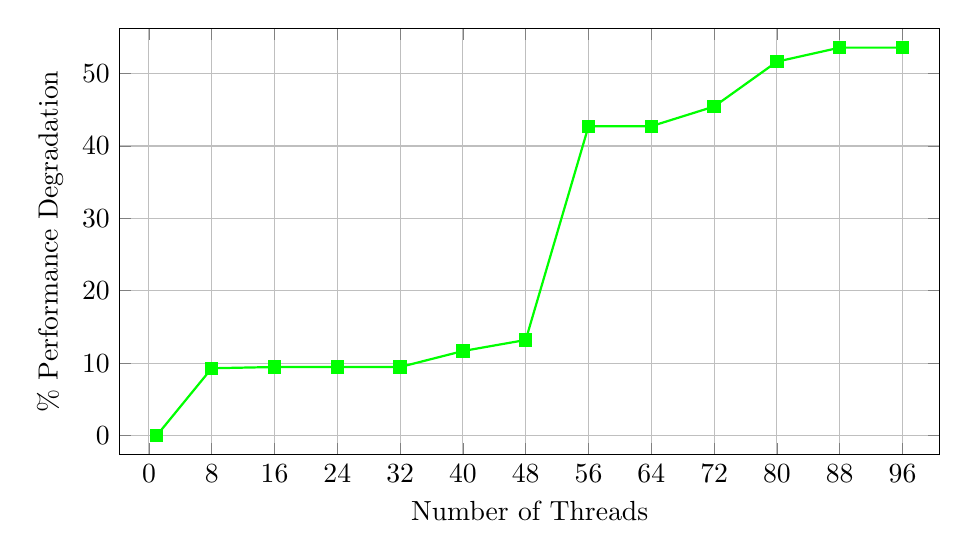
\begin{tikzpicture}
\begin{axis}[
    width=12cm,
    height=7cm,
    xlabel={Number of Threads},
    ylabel={\% Performance Degradation},
    grid=both,
    xtick distance=8,
    enlargelimits=0.05,
    legend style={at={(0.5,-0.25)}, anchor=north, legend columns=2}
]

\addplot[
    color=green,
    mark=square*,
    thick
] coordinates {
    (1, 0)
    (8, 9.29)
    (16, 9.46)
    (24, 9.47)
    (32, 9.46)
    (40, 11.67)
    (48, 13.2)
    (56, 42.74)
    (64, 42.74)
    (72, 45.46)
    (80, 51.66)
    (88, 53.6)
    (96, 53.6)
};


\end{axis}
\end{tikzpicture}
\caption{Runtime impact of incrementally increasing threads in the \textit{cpu\_burn} command on an m5.metal instance} 
\label{fig::m5_metal}
\end{figure}
\noindent
Although the m5.metal has 96 vCPUs i.e., logical cores, we 
notice a very important pattern of performance degradation throughout the first 96 threads reaching 53\%. 
This is caused by the physical core co-location that happens between the different 
threads, resulting in resource contention, as the execution resources are not duplicated. 
We also notice a very interesting point. In all our previous experiments, the instances 
initially started with a nominal baseline performance significantly worse than running the 
exact number of threads directly on the metal instance. Figure \ref{fig::metal_vs_VMs} compares 
the runtime of \textit{cpu\_burn} on the test node (all threads are busy) as we keep adding fully busy 
neighbors, in comparison to running the same number of busy threads directly on the m5.metal. 
\begin{figure}[H]
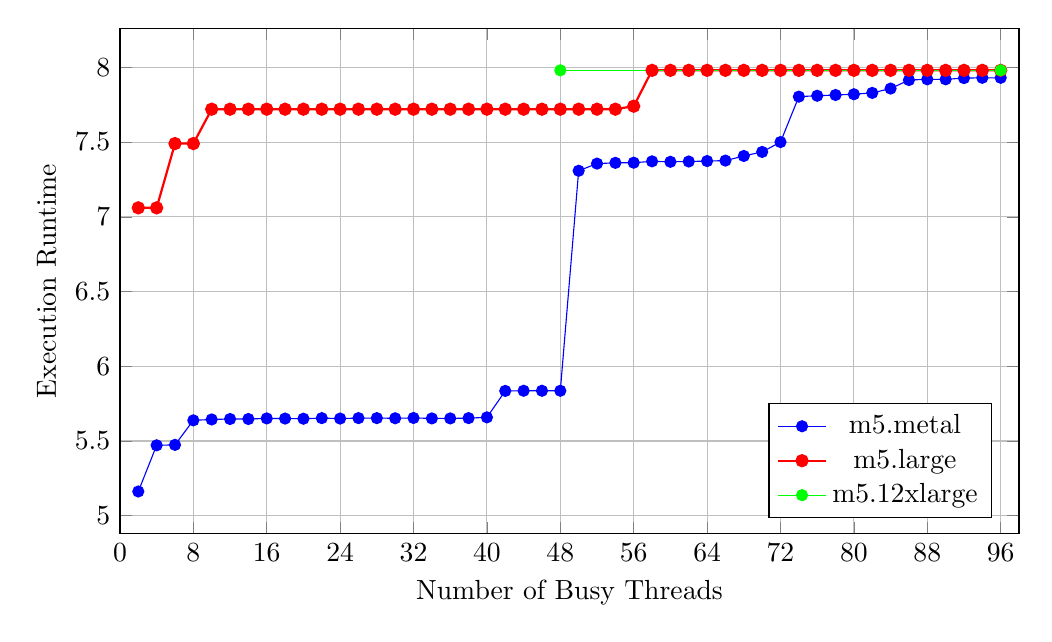
\begin{tikzpicture}
\begin{axis}[
    width=13cm,
    height=8cm,
    ylabel={Execution Runtime},
    xlabel={Number of Busy Threads},
    grid=major,
    xmin=0, 
    xmax=98,
    xtick distance= 8,
    legend pos=south east
]
\addplot[
    color=blue,
    mark=*,
] coordinates {
    (2, 5.162)
    (4, 5.471)
    (6, 5.474)
    (8, 5.638)
    (10, 5.644)
    (12, 5.647)
    (14, 5.647)
    (16, 5.651)
    (18, 5.650)
    (20, 5.649)
    (22, 5.653)
    (24, 5.650)
    (26, 5.653)
    (28, 5.653)
    (30, 5.652)
    (32, 5.654)
    (34, 5.651)
    (36, 5.651)
    (38, 5.653)
    (40, 5.658)
    (42, 5.835)
    (44, 5.836)
    (46, 5.836)
    (48, 5.836)
    (50, 7.308)
    (52, 7.356)
    (54, 7.361)
    (56, 7.362)
    (58, 7.371)
    (60, 7.368)
    (62, 7.370)
    (64, 7.373)
    (66, 7.376)
    (68, 7.407)
    (70, 7.434)
    (72, 7.5)
    (74, 7.804)
    (76, 7.81)
    (78, 7.815)
    (80, 7.82)
    (82, 7.829)
    (84, 7.858)
    (86, 7.915)
    (88, 7.92)
    (90, 7.92)
    (92, 7.928)
    (94, 7.93)
    (96, 7.93)
};

\addlegendentry{m5.metal}
\addplot[
    color=red,
    mark= *,
    thick,
] coordinates {
    (2, 7.06)
(4, 7.06)
(6, 7.49)
(8, 7.49)
(10, 7.72)
(12, 7.72)
(14, 7.72)
(16, 7.72)
(18, 7.72)
(20, 7.72)
(22, 7.72)
(24, 7.72)
(26, 7.72)
(28, 7.72)
(30, 7.72)
(32, 7.72)
(34, 7.72)
(36, 7.72)
(38, 7.72)
(40, 7.72)
(42, 7.72)
(44, 7.72)
(46, 7.72)
(48, 7.72)
(50, 7.72)
(52, 7.72)
(54, 7.72)
(56, 7.74)
(58, 7.98)
(60, 7.98)
(62, 7.98)
(64, 7.98)
(66, 7.98)
(68, 7.98)
(70, 7.98)
(72, 7.98)
(74, 7.98)
(76, 7.98)
(78, 7.98)
(80, 7.98)
(82, 7.98)
(84, 7.98)
(86, 7.98)
(88, 7.98)
(90, 7.98)
(92, 7.98)
(94, 7.98)
(96, 7.98)
 };
 \addlegendentry{m5.large}

 \addplot[
    color=green,
    mark=*,
] coordinates {
(48, 7.98)
(96, 7.98)
 };
 \addlegendentry{m5.12xlarge}
\end{axis}
\end{tikzpicture}
\caption{Performance of the test node (while incrementally adding busy neighbors) in comparison 
to running the threads natively on m5.metal}
\label{fig::metal_vs_VMs}
\end{figure}
\noindent
The first two threads finished the execution in 5.165s on the bare metal instance. However, the 
first m5.large instance that  was deployed on the dedicated host took 7.06s to 
finish, even though it introduced the first two busy threads on the dedicated host and no other VMs exists.
This is highly unexpected as we would have expected to see a runtime closer to 5.165s that confirms 
the promises of AWS of a near bare-metal performance. Instead we notice a difference of almost 36.6\%. 
The same is true for the first m5.12xlarge instance where we witness a difference of 36.7\%. Furthermore, we notice that both plots converge almost towards the same value at 
the maximum number of threads. This strongly undermines the hypothesis that the degradation is due to 
hypervisor overhead as we would expect to see an even bigger gap (in relation to bare-metal) as 
more VMs are deployed on the dedicated host. The results for the performance degradation we saw in 
the previous experiments (Table 2) can be misleading. For bigger instances, we saw a relatively small 
degradation compared to the smaller instances (large and xlarge). The reason behind this is that the 
first 12xlarge instance started with a baseline performance that's 13\% worse than the performance 
of the first m5.large instance as Figure \ref{fig::metal_vs_VMs} shows. \\
The poor initial performance of the first m5.large instance (test node) suggests that the hypervisor 
pinned its vCPUs to the same physical core, not taking advantage of other non-occupied physical cores. 
We assume that this allocation technique aims to avoid contention between the different tenants/customers 
and isolate the vCPUs of each virtual machine by allocating each pair to the same physical core. 
This could be advantageous when the customer rents a unique VM, as it is independent of the neighbors’ 
workloads. However, it is highly unfavorable when the user has access to a dedicated host, as they 
are unable to fully utilize the available idle CPU resources of the physical machine, despite paying 
for all of them. \\
To confirm our supposition, we run the \textit{cpu\_burn} tool in a m5.2xlarge instance, and incrementally 
increase the number of busy threads. The results can be seen in the following figure. 
\begin{figure}[H]
\centering
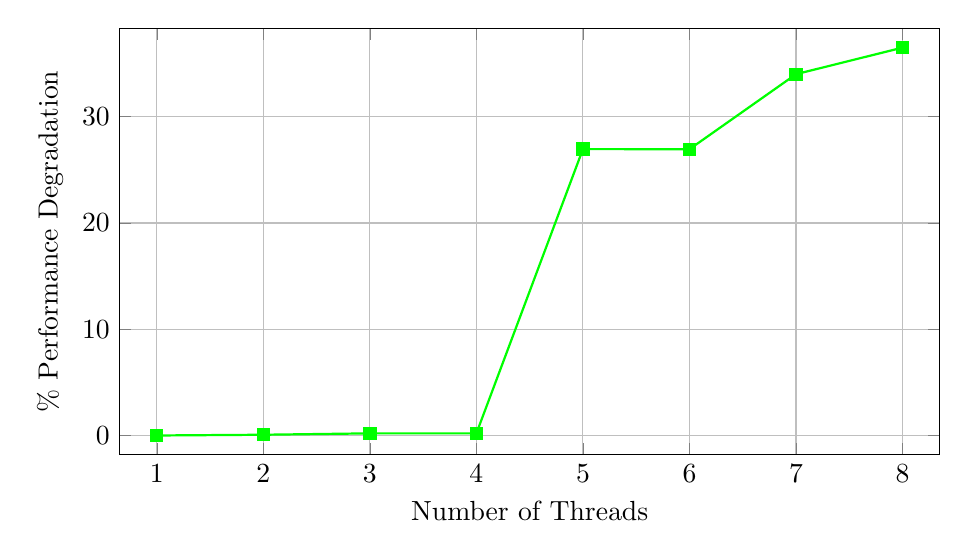
\begin{tikzpicture}
\begin{axis}[
    width=12cm,
    height=7cm,
    xlabel={Number of Threads},
    ylabel={\% Performance Degradation},
    grid=both,
    enlargelimits=0.05,
    legend style={at={(0.5,-0.25)}, anchor=north, legend columns=2}
]

\addplot[
    color=green,
    mark=square*,
    thick
] coordinates {
    (1, 0)
    (2, 0.07)
    (3, 0.2)
    (4, 0.2)
    (5, 26.95)
    (6, 26.94)
    (7, 34)
    (8, 36.5)
};


\end{axis}
\end{tikzpicture}
\caption{Effect of adding busy threads on the CPU performance of a m5.2xlarge instance using \textit{cpu\_burn}} 
\label{fig::m5_inter}
\end{figure}
\noindent
We can notice that the biggest degradation happens when adding the 5th thread, which strongly indicates 
that the instance has access to only 4 physical cores. The hypervisor starts by initially pinning the 
first 4 threads to an idle physical core to maximize performance but then the 5th thread is allocated 
to one of these physical cores, sharing the execution resources with another busy thread resulting in 
a performance degradation of 27\%.  \\
\subsubsection{Performance variation of random m5.large instances}
We wanted to analyze the variation of the performance of different m5.large instances. For this we 
sequentially launched 50 m5.large instances across different zones of the us-east-2 region to see where their 
execution runtime is situated in relation to figure \ref{fig::metal_vs_VMs}. The runtime across all the subjects
was consistently 7.98 seconds. This consistency strongly suggests that AWS pre-provisions idle instances on 
internally managed dedicated hosts even before they're rented, enabling faster boot times 
when a customer actually rents a VM. If this were not the case, then we would have expected to see 
execution runtimes around  7, 7.5 or 7.7 seconds which correspond to the three performance 
levels we witnessed on figure \ref{fig::metal_vs_VMs}. 
